
\documentclass[12pt]{article}

% Layout.
\usepackage[top=1in, bottom=0.75in, left=1in, right=1in, headheight=1in, headsep=6pt]{geometry}

% Fonts.
\usepackage{mathptmx}
\usepackage[scaled=0.86]{helvet}
\renewcommand{\emph}[1]{\textsf{\textbf{#1}}}

% TiKZ.
\usepackage{tikz, pgfplots}
\usetikzlibrary{calc}
\pgfplotsset{compat = newest}
 
\pgfplotsset{my style/.append style={axis x line=middle, axis y line=
middle, xlabel={$x$}, ylabel={$y$}, axis equal
}}

% Misc packages.
\usepackage{amsmath,amssymb,latexsym}
\usepackage{graphicx}
\usepackage{array}
\usepackage{xcolor}
\usepackage{multicol}

% Commands to set various header/footer components.
\makeatletter
\def\doctitle#1{\gdef\@doctitle{#1}}
\doctitle{Use {\tt\textbackslash doctitle\{MY LABEL\}}.}
\def\docdate#1{\gdef\@docdate{#1}}
\docdate{Use {\tt\textbackslash docdate\{MY DATE\}}.}
\def\doccourse#1{\gdef\@doccourse{#1}}
\let\@doccourse\@empty
\def\docscoring#1{\gdef\@docscoring{#1}}
\let\@docscoring\@empty
\def\docversion#1{\gdef\@docversion{#1}}
\let\@docversion\@empty
\makeatother

% Headers and footers layout.
\makeatletter
\usepackage{fancyhdr}
\pagestyle{fancy}
\fancyhf{} % Clears all headers/footers.
\lhead{\baselineskip 30pt
%\emph{\@doctitle\hfill\@docdate}
\emph{\@docdate\hfill\@doctitle}
\ifnum \value{page} > 1\relax\else\\
\emph{Name: \rule{3.5in}{1pt}\hfill \@docscoring}\fi}
\rfoot{\emph{\@docversion}}
\lfoot{\emph{\@doccourse}}
\cfoot{\emph{\thepage}}
\renewcommand{\headrulewidth}{0pt}%
\makeatother

% Paragraph spacing
\parindent 0pt
\parskip 6pt plus 1pt

% A problem is a section-like command. Use \problem{5} to
% start a problem worth 5 points.
\newcounter{probcount}
\newcounter{subprobcount}
\setcounter{probcount}{0}
\newcommand{\problem}[1]{%
\par
\addvspace{4pt}%
\setcounter{subprobcount}{0}%
\stepcounter{probcount}%
\makebox[0pt][r]{\emph{\arabic{probcount}.}\hskip1ex}\emph{[#1 points]}\hskip1ex}
\newcommand{\thesubproblem}{\emph{\alph{subprobcount}.}}

% Subproblems are an enumerate-like environment with a consistent
% numbering scheme. 
% Use \begin{subproblems}\item...\item...\end{subproblems}
\newenvironment{subproblems}{%
\begin{enumerate}%
\setcounter{enumi}{\value{subprobcount}}%
\renewcommand{\theenumi}{\emph{\alph{enumi}}}}%
{\setcounter{subprobcount}{\value{enumi}}\end{enumerate}}

% Blanks for answers in normal and math mode.
\newcommand{\blank}[1]{\rule{#1}{0.75pt}}
\newcommand{\mblank}[1]{\underline{\hspace{#1}}}
\def\emptybox(#1,#2){\framebox{\parbox[c][#2]{#1}{\rule{0pt}{0pt}}}}

% Misc.
\renewcommand{\d}{\displaystyle}
\newcommand{\ds}{\displaystyle}
\def\bc{\begin{center}}
\def\ec{\end{center}}
\def\be{\begin{enumerate}}
\def\ee{\end{enumerate}}


\doctitle{Math 251: Quiz 3}
\docdate{Jan 27, 2022}
\doccourse{UAF Calculus I}
\docversion{v-1}
\docscoring{\blank{0.8in} / 25}
\begin{document}
%\textbf{Please circle your instructor's name:} \hfill Leah Berman  \hfill   Jill Faudree\\

There are 25 points possible on this quiz. No aids (book, calculator, etc.)
are permitted.  {\bf Show all work for full credit.}

\problem{11} Use the graph of the function $H(x)$ (drawn below) to answer the questions. Assume $H(x)$ has a vertical asymptote at $x=4.$ For each problem below, give the most complete answer; if the limit is infinite, indicate that with $\infty$ or $-\infty.$ If a value does not exist, write DNE.\\

\begin{center}
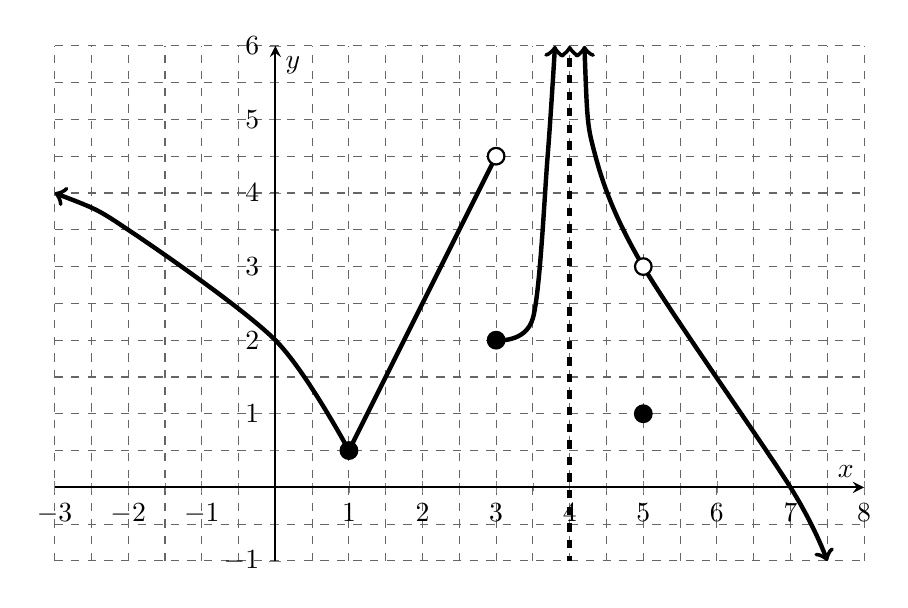
\begin{tikzpicture}
\begin{axis}[scale=1.5, thick, my style, xtick={-3,...,8}, ytick={-1, 0,...,6},
xmin=-3, xmax=8, ymin=-1, ymax=6, minor y tick num=1,
        minor x tick num=1, mark size=3.0pt, grid=both, grid style={ thin, black!60, dashed}, axis equal image
        ]
% %%asymptote
\addplot[dashed,<->, ultra thick] coordinates {(4,-2) (4,6)};       
%%points solid
\addplot[mark=*,only marks] coordinates {(3,2)(5,1) (1,0.5)};
%%points open
\addplot[mark=*,fill=white,only marks] coordinates {(3,4.5)(5,3)};
%%Curves
\addplot[ultra thick, smooth,<-] coordinates {(-3,4) (-2,3.5) (0,2)(1,0.5)};
\addplot[ultra thick, smooth] coordinates {(1,0.5) (3,4.5)};
\addplot[ultra thick, smooth,->] coordinates {(3,2) (3.5,2.3) (3.7,4.5) (3.8,6)};
\addplot[ultra thick, smooth,<->] coordinates {(4.2,6) (4.35,4.5) (5,3) (7,0) (7.5,-1)};       
\end{axis}
\end{tikzpicture}
\end{center}

\begin{subproblems}
\begin{multicols}{3}
\item $f(1)=\mblank{.5in}$
\item $f(3)=\mblank{.5in}$
\item $f(5)=\mblank{.5in}$
%\item $f(5)=\mblank{.5in}$
\end{multicols}
\vspace{0.1in}
\begin{multicols}{3}
\item $\d{\lim_{x \to\; 3^-} f(x)=\mblank{.5in}}$
\item $\d{\lim_{x \to\; 3^+} f(x)=\mblank{.5in}}$
\item $\d{\lim_{x \to\; 3} f(x)=\mblank{.5in}}$
\end{multicols}
\vspace{0.1in}
\begin{multicols}{3}
\item $\d{\lim_{x \to 4} f(x)=\mblank{.5in}}$
\item $\d \lim_{x\to\; 5}f(x)=\mblank{.5in}$
\item $\d{\lim_{x \to 7} f(x)=\mblank{.5in}}$
\end{multicols}
\vspace{0.1in}
\item List all $x$-values for which the function $H(x)$ fails to be continuous.\\
\vfill

\end{subproblems}
\newpage
\problem{10} Evaluate the following limits. Give the most complete answer; if the limit is infinite, indicate that with $\infty$ or $-\infty.$ If a value does not exist, write DNE. You must show work to receive full credit.\\
\begin{subproblems}
\item $\d{\lim_{ x\to 4} \frac{2x^2-8x}{x^2-x-12}}$ 
\vfill
\item $\d{\lim_{ x\to 1} \frac{\sqrt{3+x}-2}{x-1}}$ 
\vfill
\item $\d{\lim_{ x\to -2^+} \frac{5x}{x+2}}$ 
\vfill
\item Given $\d{\lim_{ x \to 10} f(x) = 5}$ and $\d{\lim_{ x \to 10} g(x) = -3}$, evaluate $\displaystyle{\lim_{ x \to 10}\; 2\left(\frac{x+1}{f(x)+g(x)}\right)}.$ 
\vspace{.5in}
\end{subproblems}

\problem{4} Use the Intermediate Value Theorem to show that the polynomial $p(x)=x^3-x+2$ must reach a $y$-value of $5$ for some $x$-value on the interval $[1,2].$ \\
\vfill
\end{document}